\documentclass[%
 reprint,
 amsmath,
 amssymb,
 aps,
 floatfix,
]{revtex4-2}


\usepackage{graphicx}% Include figure files
\usepackage{dcolumn}% Align table columns on decimal point
\usepackage{bm}% bold math
\usepackage{lipsum}
\usepackage{physics}
\usepackage{xcolor}


\bibliographystyle{apsrev4-2}

\begin{document}

\title{Parity Partner Bands in $^{163}$Lu: \\ A novel approach in describing the negative parity states from its wobbling spectrum}% Force line breaks with \\

\author{Robert Poenaru}%
 \email{robert.poenaru@drd.unibuc.ro}
 \affiliation{Doctoral School of Physics, University of Bucharest}%
 \affiliation{Horia Hulubei National Institute of Nuclear Physics and Engineering, Magurele}%
\author{Apolodor Aristotel Raduta}%
\affiliation{Horia Hulubei National Institute of Nuclear Physics and Engineering, Magurele}%
\affiliation{Academy of Romanian Scientists, Bucharest}%

\date{\today}

\begin{abstract}
The wobbling spectrum of $^{163}$Lu is described through a novel approach, starting from a triaxial rotor model within a semi-classical picture, and obtaining a new set of equations for all four rotational bands that have wobbling character. Redefining the band structure in the present model is done by adopting the concepts of Signature Partner Bands and Parity Partner Bands. Indeed, describing a wobbling spectrum in a even-odd nucleus through signature and parity quantum numbers is a unique interpretation of the triaxial super-deformed structures in the chart of nuclides.
\end{abstract}

\maketitle


%\section{Introduction}

Triaxiality in nuclear systems represented a great challenge over the last decades for the Nuclear Physics community due to its elusive character, however, a tremendous progress has been made in the recent years, both theoretically and experimentally. Regarding its fingerprints, it is a widely known and accepted fact that the phenomenon of \emph{Wobbling Motion} (WM) is a clear signature for triaxial shapes across the chart of nuclides. Although it was firstly predicted theoretically for even-even nuclei \cite{bohr1998nuclear}, this collective mode has been discovered and confirmed experimentally in several even-odd nuclei, with $^{163}$Lu being considered the best \emph{wobbler}, mainly due to its relatively rich spectrum in terms of wobbling bands (with four triaxial super-deformed bands TSD1,2,3, and 4, with TSD1 as the ground state - yrast - band and three wobbling excitations). Indeed, it was shown \cite{odegaard2001evidence}, \cite{jensen2002wobbling} that stable triaxial shapes occur in this isotope due to the aligned $i_{13/2}$ proton which drives the nucleus up to very large deformation. With time, several neighboring nuclei were identified as wobblers (i.e., $^{161,165,167}$Lu, and recently the nuclei $^{135}$Pr \cite{matta2017transverse,sensharma2019two} and $^{187}$Au \cite{sensharma2020longitudinal}).

Within a previous model \cite{raduta2020towards}, a description of the wobbling phenomenon in $^{163}$Lu was successfully made, describing the wobbling energies and the transition probabilities for all four triaxial super-deformed (TSD) bands, namely TSD1, TSD2, TSD3, and TSD4. Therein, the calculations were based on a particle-triaxial rotor that was solved on a semi-classical formalism. The band structure was described in terms of two ground states given by the coupling of the core with an odd $j=i_{13/2}$ proton, one excited wobbling band $n_w=1$ from the coupling of the core with the same proton, and one ground state band obtained from the coupling of the core and a different valence nucleon, namely the $j=h_{9/2}$ nucleon. More precisely, the TSD1 and TSD2 are considered as ground states (with zero wobbling phonon excitations) for the nucleus, with TSD1 made up of a spins sequence $\mathbf{I}=\mathbf{R}+\mathbf{j}$ with the core's angular momentum as an even integer sequence $\mathbf{R}=0,2,4,\dots$ and TSD2 is a spin sequence generated from a core-particle-coupling with odd integer spin of the core $\mathbf{R}=1,3,5,\dots$. TSD3 has indeed a wobbling phonon character, and it is obtained by exciting the states belonging to TSD2 by a specific one phonon operator. As mentioned, TSD4 consists in a collection of energies that emerge from the core's coupling with a a valence nucleon from a different $j$-shell (i.e., $j=h_{9/2}$). In terms of the TSD4 ground state band, the spin sequence $\mathbf{I}=\mathbf{R}+\mathbf{j}$ has odd integers for the core's angular momentum $\mathbf{R}=1,3,5,\dots$, just like the TSD2.

It is worth mentioning some key points from \cite{raduta2020towards} and \cite{raduta2020new} that would be relevant as a starting point for the present study. i) Indeed, in the mentioned work it was shown that TSD1 and TSD2 are signature partner bands \cite{sun1994varied}, with the yrast band being characterized by positive signature number $\alpha=1/2$ (favored partner), while the second band has negative signature $\alpha=-1/2$ (unfavored partner). The signature quantum number is specific to deformed nuclei, and moreover it indicates the invariance of a nuclear system with quadrupole deformation under rotations with $\pi$ around the principal axes (with the observation that if the nucleus has axial symmetry, then the only rotations around the principal axes other than the symmetry one can have a good signature quantum number). Potential energy calculations that were performed for the case even-odd triaxial nuclei within \cite{raduta2016specific}-\cite{raduta2017semiclassical}, show that the minima are deep, so that states from TSD2 cannot tunnel to a secondary minimum, as a result, both bands share similar properties. ii) The fourth band in $^{163}$Lu was reconsidered as a zero-phonon wobbling excitation, since it belongs to a different coupling scheme and that also reflected in the calculations regarding the excitation energies of its states. More precisely, a different sets of moments of inertia, triaxiality parameter, and single-particle potential strength had to be considered in the numerical calculations, since the triaxial-core-coupling differed from that of TSD1,2 and 3 (see Eq. (12) in \cite{raduta2020new}). iii) Calculations regarding the stationary points of the energy function associated to the triaxial even-odd nucleus lead to the possibility to construct a phase diagram, which could show regions where both longitudinal and transverse wobbling character might occur, but also regions in that space were wobbling motion is forbidden. In fact, within those calculations, the model was able to predict that transverse wobbling is possible, but in an \emph{intermediate} picture, where the longitudinal character emerges as a final collective mode, from a state where the deformed system rotates around the $m$-axis. However, this is a limitation of the used Hamiltonian, and Appendix B from \cite{raduta2020new} shows that for spin-dependent moments of inertia and Coriolis-like interaction it is possible to consistently reproduce a decreasing wobbling energy as a function of rotational frequency or spin, specific to a transverse-like character of the WM. iv) The used formalism applied to the study of $A=163$ Lu isotope is not based on microscopic calculations which could justify the fact that fourth band has negative parity $\pi_4=-1$. As a matter of fact, the parity of the odd system is given by the product of parities associated to the core and the single particle (i.e., positive parity attributed to the core and negative parity that is attributed to the valance nucleon). From a microscopic point of view, the particle-hole excitations involve one positive single parity state that belongs to the core and one negative parity that belongs to the odd-particle.

Starting from the model sketched above, some further investigations on the actual band structure of $^{163}$Lu had been developed, with a focus on the energy spectrum, and whether it is possible to give a proper interpretation of the parity of all four bands. Namely, a great interest was given to TSD4, in order to see if its coupling might be strongly related to the first three bands. As such, an attempt on describing the excited states from TSD4 by adopting the same $\mathbf{I}=\mathbf{R}+\mathbf{j}$ coupling scheme as for TSD2 (where the valence nucleon from the $i_{13/2}$ orbital is coupled to the even-even triaxial core) is made in this paper. Results show that TSD2 and TSD4 are \emph{parity partner bands}, where they both have the same core spin sequence $\mathbf{R}=1,3,5,\dots$ but opposite parity numbers; $\pi_4=-\pi_2$. The concept of (negative) parity for even-even and even-odd deformed nuclei has been extensively studied over the last years (See Refs. \cite{raduta2006description}, \cite{raduta2006positive}, \cite{raduta2006simultaneous}, and \cite{bizzeti2008description}). 

Parity number $\pi$ describes the symmetry of the underlying Hamiltonian under a space reflection operation. Moreover, it is suggested that negative parity band structures in nuclei might be related to the existence of octupole deformations \cite{chasman1980incipient},\cite{asaro1953complex}. However, no concrete evidence that the states belonging to TSD4 could lead to pear shaped nuclear surfaces in $^{163}$Lu has been found so far. As a result, the present work asserts the possibility that indeed TSD4 belongs to the same family of wobbling bands as the previous three (enforced by the calculations that show similar behavior of the dynamic moment of inertia, alignment and the electromagnetic transitions performed by the same team in \cite{raduta2020towards}), while the pair (TSD2,TSD4) emerge as a collection of states with similar spins but opposite parity. This implies that due to a similar coupling scheme between $\mathbf{R}$ and $\mathbf{j}$ across all four bands (as opposed to previous models that considered the triaxial core+odd $j=h_{9/2}$ coupling) , a similar set of moments of inertia can be attributed within the calculations regarding the energies of the states, and moreover, the nucleus has the same triaxiality parameter $\gamma$, while the valence nucleon (that is the odd proton from $i_{13/2}$ orbital) is moving in a quadrupole deformed mean field generated by the core, with the same strength parameter $V$ \cite{shou2009coupling}. In fact, the present model considers these quantities as free parameters and they represent an unique set associated with all four bands. Numerical calculations will determine the values for the MOIs $\mathcal{I}_1$, $\mathcal{I}_2$, $\mathcal{I}_3$, $\gamma$ and $V$ (four free parameters) in such a way that the energy spectrum obtained will consistently reproduce the experimental data.

Regarding the nature of the bands TSD1 and TSD3, in the present model they remain unchanged. More precisely, the yrast band with zero-phonon excitation TSD1 that emerges as a collection of states with even-numbers for the core's spin sequence, and the one-wobbling-phonon excitation band TSD3 with a state $I$ which is built on top of TSD2 by acting on a $(I-1)\in \text{TSD2}$ state with a phonon operator.

Further investigations using this novel approach were devoted to the study of nuclear motion for even-odd triaxial systems. Working within a semi-classical picture allows one to keep a close contact with the classical features of the nuclear system dynamics, and to have a consistent description with the motion of a nucleus and that of a classical rigid rotor. Several studies \cite{frauendorf2014transverse}, \cite{lawrie2020tilted} showed the \emph{trajectories} of a simple rotor for a given total angular momentum and inertia parameters of the triaxial ellipsoid. One can view these trajectories as the allowed states of existence which the isotope might have with the increase in angular momentum. They are generated by the motion of the angular momentum vector, which from a classical point of view, it is the intersection of the angular momentum sphere and that of the energy ellipsoid. From the conservation of these two quantities, it is possible to extract information with regards to the intersection lines within the angular momentum space, and even predict certain trajectories with larger rotational spin and energy.
 


%\section{Theoretical Framework}

The Hamiltonian of $^{163}$Lu has a particle-rotor character, namely it describes the interaction between an even-even triaxial core and a single nucleon that moves in the quadrupole deformed mean field generated by the core.

\begin{align}
    H=H_\text{Rot}+H_\text{sp}\ . \label{hamiltonian_formula}
\end{align}

The first term represents the triaxial rotor Hamiltonian that is associated with the core angular momentum $\mathbf{R}=\mathbf{I}-\mathbf{j}$, and it is defined by the inertial parameters $A_k$.

\begin{align}
    H_\text{Rot}=\sum_{i=1,2,3}A_i\left(I_i-j_i\right)^2,
\end{align}
 
 where the inertial parameters $A_i$ are related to the moments of inertia through the formula $A_i=\frac{1}{2\mathcal{I}_i}$. The moments of inertia are associated to the principal axes of the triaxial ellipsoid, namely the $i$-th MOI $\mathcal{I}_i$ corresponds to the $i$-axis of the system.

The single-particle term from Eq. \ref{hamiltonian_formula} is defined in terms of the triaxiality parameter $\gamma$, which defines the ratios between MOIs and it is a measure of asymmetry, and the potential strength $V$, that is related to the deformation of quadrupole type (in \cite{shou2009coupling}, a determination of the interaction parameter $V$ is determined in terms of the quadrupole deformation $\beta_2$ using the single-$j$ shell model).

\begin{align}
    H_\text{sp} = \frac{V}{j(j+1}\left[\cos\gamma\left(3j_3^2-\mathbf{j}^2\right)-\sqrt{3}\sin\gamma\left(j_1^2-j_2^2\right)\right]+\epsilon_j. \label{sp_hami}
\end{align}

The term $\epsilon_j$ from Eq. \ref{sp_hami} represents the single particle energy associated with the orbital from which the valence nucleon belongs to.

With the above Hamiltonian, and by following the recipe described in Section II from \cite{raduta2020new}, it is possible to obtain a set of classical equations of motion for $\mathcal{H}$ - the classical energy, defined as the expectation value of $H$ with the trial function used throughout the calculations (See Eqs. (1)-(9) from \cite{raduta2020new}). The energy function $\mathcal{H}$ is minimal in the point $(\varphi,r;\psi,t)=(0,I;0,j)\equiv P_0$ when the maximal moment of inertia for the triaxial nucleus is along the 1-axis. A harmonic motion of the system is obtained if one linearizes the equations of motion around $P_0$, with the frequency of the motion given by a dispersion equation, which under the restrictions $\mathcal{I}_1>(\mathcal{I}_2,\mathcal{I_3})$ admits two real and positive solutions. These solutions represent the \emph{wobbling frequencies} $\Omega_1$ and $\Omega_2$ that will be used for the analytic expressions of the excited spectrum of $^{163}$Lu. The notations used in the previous model differ from the current one, since there were two cases for consideration, namely the coupling of the core with $j_1=i_{13/2}$ and with $j_2=h_{9/2}$. Here, for simplicity, differentiation between the two frequencies will be done the indexes 1,2, but both solutions are associated to the unique $\mathbf{R}+\mathbf{j}$ coupling for all four TSD bands where $j=j_1$. In \cite{raduta2017semiclassical} it was shown that the solutions of the dispersion equation for $\Omega$ correspond to the motion of the core ($\Omega_1$) and the odd-particle ($\Omega_2$), and moreover, each wobbling quanta has a corresponding wobbling phonon number $n_{w_1}$ and $n_{w_2}$, respectively. Having thus the minimal energy $\mathcal{H}_min$ (given as the classical energy function evaluated at $P_0$ for a given total angular momentum), and the two wobbling frequencies (given as solutions to the dispersion equation associated to the harmonic motion of the system) with their corresponding wobbling phonon numbers, the energy spectrum of the studied isotope can be defined as:

\begin{align}
    E_I^\text{TSD1}=\epsilon_{j_1} + \mathcal{H}_\text{min}^{(I,j_1)}+\mathcal{F}_{00}^I \nonumber\ ,\\
    E_I^\text{TSD2}=\epsilon_{j_1} + \mathcal{H}_\text{min}^{(I,j_1)}+\mathcal{F}_{00}^I \nonumber\ ,\\
    E_I^\text{TSD3}=\epsilon_{j_1} + \mathcal{H}_\text{min}^{(I,j_1)}+\mathcal{F}_{10}^I \nonumber\ ,\\
    E_I^\text{TSD4}=\epsilon_{j_1} + \mathcal{H}_\text{min}^{(I,j_1)}+\mathcal{F}_{00}^I \label{wobbling_energies}
\end{align}

where the terms $\mathcal{F}_{n_{w_1}n_{w_2}}$ represent the wobbling frequencies of phononic character, associated to each band. These terms are related to the total angular momentum through the following expression:

\begin{align}
    F_{n_{w_1}n_{w_1}}^I=\frac{1}{2}\left(n_{w_1}\Omega_1^I+n_{w_2}\Omega_2^I\right) \label{phonons}
\end{align}

with the observation that for TSD2 and TSD4, due to their interpretation as being parity partners, a \emph{shift} in the overall energy will appear (denoted hereafter with $\epsilon_2$ for TSD2 and $\epsilon_4$ for TSD4) for each band. These two quantities will be adjusted throughout the numerical calculations such that the energy spectrum is best reproduced. From the expression of Eq. \ref{phonons}, one can see what wobbling phonon numbers are associated to the frequencies, for each of the triaxial bands. These values are listed in the Table \ref{tabular_phonon_numbers}, where values of the parity and signatures are also shown. The spin sequences for the triaxial bands are shown in Table \ref{spin_sequences}.

\begin{table}[h]
    \centering
  \begin{tabular}{lllll}
  \hline
Band & $n_{w_1}$ & $n_{w_2}$ &  $\pi$ &  $\alpha$ \\
\hline
\hline
TSD1 &     0      &       0    &    +1  &    +1/2      \\
TSD2 &    0       &       0    &    +1    &        -1/2  \\
TSD3 &     1      &     0      &    +1   &        +1/2  \\
TSD4 &     0      &     0      &    -1   &     +1/2    \\
\hline
\end{tabular}
    \caption{The wobbling phonon numbers, parities and signatures assigned for the triaxial bands in $^{163}$ within the model.}
    \label{tabular_phonon_numbers}
\end{table}

\begin{table}[h]
    \centering
  \begin{tabular}{llll}
  \hline
Band & j & $\mathbf{R}$-sequence & $\mathbf{I}$-sequence \\
\hline
\hline
TSD1 & $j_1$  &   $0,2,4,\dots$         &   $13/2,17/2,21/2,\dots$         \\
TSD2 & $j_1$  &   $1,3,5,\dots$         &           $27/2,31/2,35/2,\dots$ \\
TSD3 & $j_1$  & - & $33/2,37/2,41/2,\dots$     \\
TSD4 & $j_1$  &         $1,3,5,\dots$   &       $47/2,51/2,55/2,\dots$    
\end{tabular}
    \caption{The spin sequences that belong to the wobbling spectrum of $^{163}$Lu, where $j_1$ is the $i_{13/2}$-odd proton. \emph{Observation:} since TSD3 states are obtained as wobbling phonon excitations from TSD2, there is no $\mathbf{R}$ sequence.}
    \label{spin_sequences}
\end{table}

Regarding the energy function $\mathcal{H}$, it is worth analyzing its behavior for a given angular momentum. If one considers the total spin $I$ of the nucleus described as a vector in the 3-dimensional space generated by the components of the angular momentum $I_k\equiv x_k\ ,\ k=1,2,3$. By changing the system from Cartesian to spherical coordinates, the expressions of the angular momentum components are readily obtained:

\begin{align}
    x_1=I\sin\theta \cos\varphi\ ,
    x_2=I\sin\theta \sin\varphi\ ,
    x_3=I\cos\theta.
\end{align}

In spherical coordinates, the expression of the energy function within the present case is given by the formula:

\begin{align}
    \mathcal{H}=&I\left(I-\frac{1}{2}\right)\left(A_1\cos^2\varphi+A_2\sin^2\varphi-A_3\right)-\\
    &-2A_1Ij\sin\theta+T_{rot}+T_{sp}\ , \label{energy_function}
\end{align}

where the two last terms are independent of the coordinates:

\begin{align}
    T_{rot}&=\frac{I}{2}(A_1+A_2)+A_3I^2\ ,\\
    T_{sp}&=\frac{j}{2}(A_2+A_3)+A_1j^2-V\frac{2j-1}{j+1}\sin\left(\gamma+\frac{\pi}{6}\right)\ .
\end{align}

For fixed values of angular momentum, moments of inertia, triaxiality parameter, and the single particle potential strength, one can numerically determine the values of $\mathcal{H}(\theta,\varphi)$ in the coordinate space $(\theta,\varphi)$ at constant spin $I$. By studying the stationary points of $\mathcal{H}$, one can find the set of points $(\theta_k,\varphi_k)$ for which the Hessian associated to the energy function is positive. These kind of points represent extreme values that are minimum of $\mathcal{H}$, for a given angular momentum. Such points are of interest since they lead to different wobbling character that might occur in the isotope.

The classical orbits (trajectories) of the nucleus are determined from the intersection of the angular momentum sphere with the energy ellipsoid of the total triaxial system. As in \cite{frauendorf2014transverse}, from the conservation of the total energy and the angular momentum, one can write:

\begin{align}
    I^2=&x_1^2+x_2^2+x_3^3\ ,\\
    E=&I'A_1x_1^2+I'A_2x_2^2+\left[I'A_3+A_1\frac{j}{I}\right]x_3^2+ \nonumber \\
    &+\frac{I}{2}(A_1+A_2)+A_3I^2+\frac{j}{2}(A_2+A_3)+A_1j^2- \nonumber \\
    &-I\left(I-\frac{1}{2}\right)A_3-2A_1Ij \label{ellipsoid_rotation}
\end{align}

Note that the Cartesian expressions of the energy ellipsoid and angular momentum components were used for the trajectories. For a given total angular momentum and the inertia parameter, it is possible to represent the trajectories of the deformed system, which represent the possible states with wobbling character.

%\section{Numerical results}

As a first step for testing this new interpretation, the energy spectrum corresponding to the wobbling character of $^{163}$Lu was studied. By using the energies given by Eq. \ref{wobbling_energies}, and by introducing the values shown in Table \ref{tabular_phonon_numbers}, a least squares fitting procedure was applied, for finding the parameter set $\mathcal{P}=(\mathcal{I}_1,\mathcal{I}_2,\mathcal{I}_3,\gamma,V)$, such that the deviations of the theoretical values from the experimental ones \cite{odegaard2001evidence} are minimal. Thus, it was possible to find the numerical values of $\mathcal{P}$, with the results shown in Table \ref{parameter_set}. The obtained RMS value is $\approx 80$ KeV, which is much better than that obtained through the previous model. Keep in mind that the fitting procedure was done for all four bands simultaneously, rather than finding a separate parameter set only for TSD4 (as it was the case for the work in \cite{raduta2020new}). In order to get this good agreement with the experimental data, the shifts in energies that were previously mentioned (see Eq. \ref{phonons}) were fixed to the following values: $\epsilon_2=0.3$ and $\epsilon_4=0.6$ MeV respectively. The obtained results are shown in Fig. \ref{tsd_bands}.

\begin{table}[h]
    \centering
  \begin{tabular}{lllll}
  \hline
$\mathcal{I}_1$ [$\hbar^2$/MeV] & $\mathcal{I}_2$ [$\hbar^2$/MeV]& $\mathcal{I}_3$ [$\hbar^2$/MeV] & $\gamma$ [deg.] & $V$ [MeV] \\
\hline
\hline
72              & 15              & 7               & 22       & 2.1
\end{tabular}
    \caption{The parameter set $\mathcal{P}$ that was determined by a fitting procedure of the excitation energies of $^{163}$Lu.}
    \label{parameter_set}
\end{table}

\begin{figure}
    \centering
    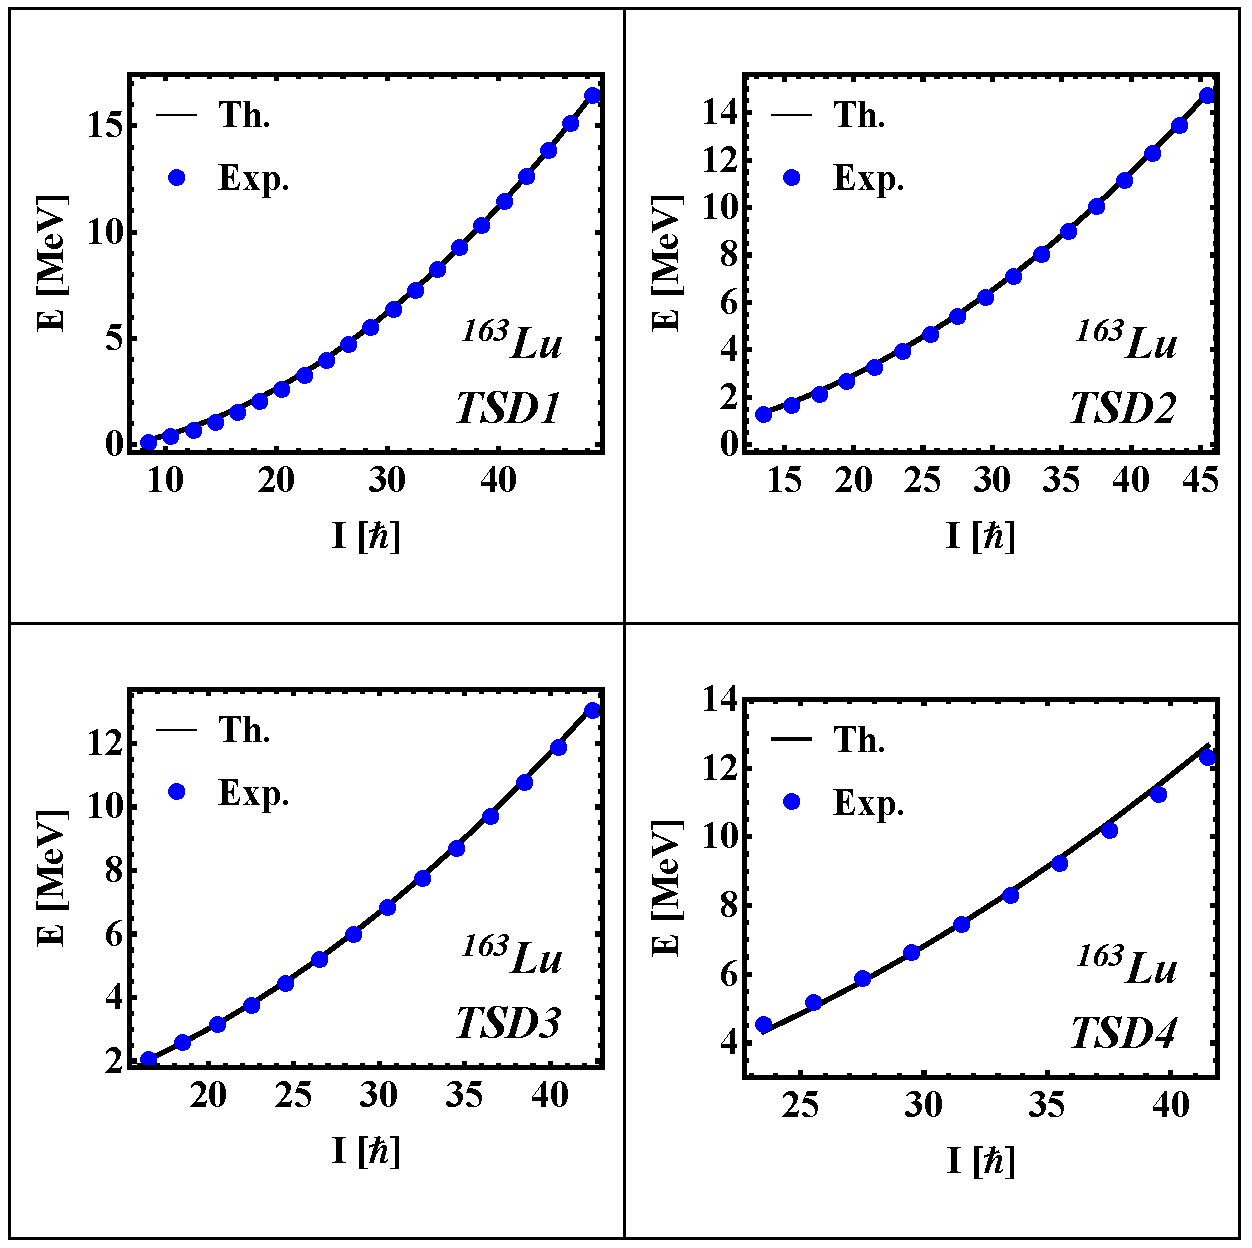
\includegraphics[scale=0.40]{images/ExcitationEnergies_GridView.pdf}
    \caption{The excitation energies for the bands TSD1, TSD2, TSD3, and TSD4.}
    \label{tsd_bands}
\end{figure}

In terms of the stability of the wobbling motion with respect to the total angular momentum, several contour plots were plotted, using the obtained parameter set $\mathcal{P}$ with the help of Eq. \ref{energy_function}. For each band, a spin close to the band head of each sequence was chosen. Due to the obtained MOI ordering, the surfaces have minimum points indicated by the red dots for each figure. Results can be seen in Figs. \ref{contour-tsd1},\ref{contour-tsd3}. Similar calculations were performed using a classical approximation for $^{135}$Pr by the same team in \cite{raduta2021}.

\begin{figure}
    \centering
    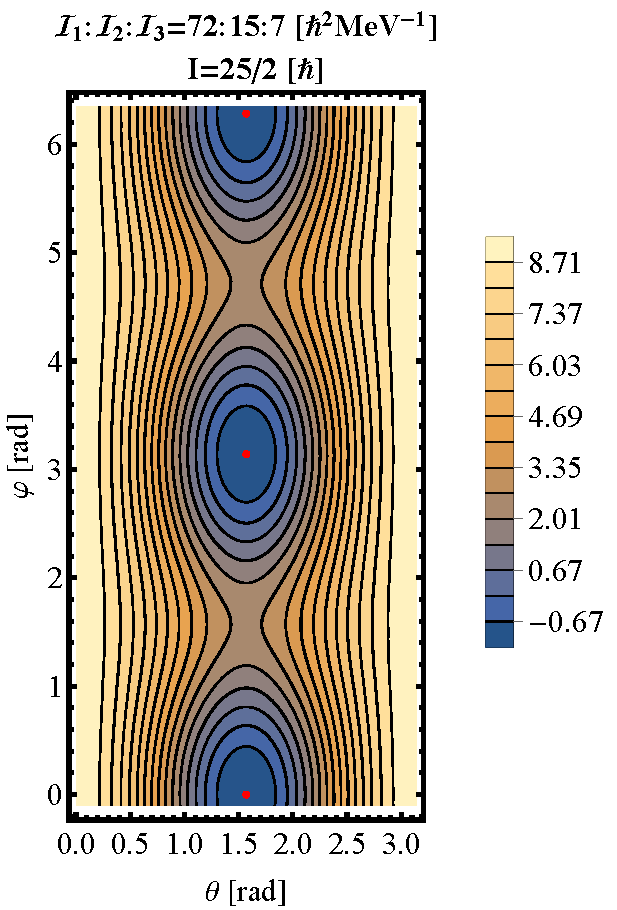
\includegraphics[scale=0.55]{images/contour-tsd1.pdf}
    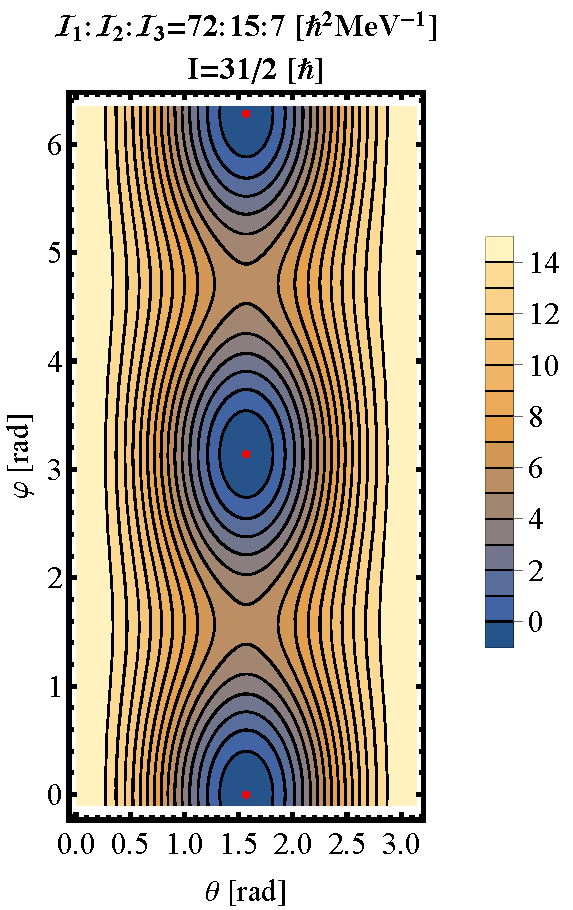
\includegraphics[scale=0.55]{images/contour-tsd2.pdf}
    \caption{A contour plot with the energy function $\mathcal{H}$ for TSD1 and TSD2. The parameter set $\mathcal{P}$ was used for the numerical calculations.}
    \label{contour-tsd1}
\end{figure}

% \begin{figure}
%     \centering
%     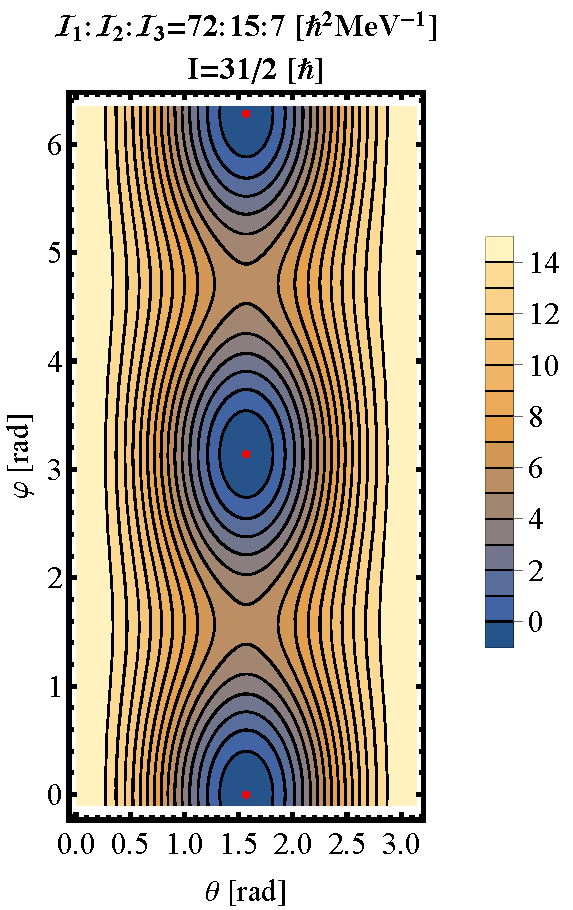
\includegraphics[scale=0.55]{images/contour-tsd2.pdf}
%     \caption{A contour plot with the energy function $\mathcal{H}$ for TSD2. The parameter set $\mathcal{P}$ was used for the numerical calculations.}
%     \label{contour-tsd2}
% \end{figure}

\begin{figure}
    \centering
    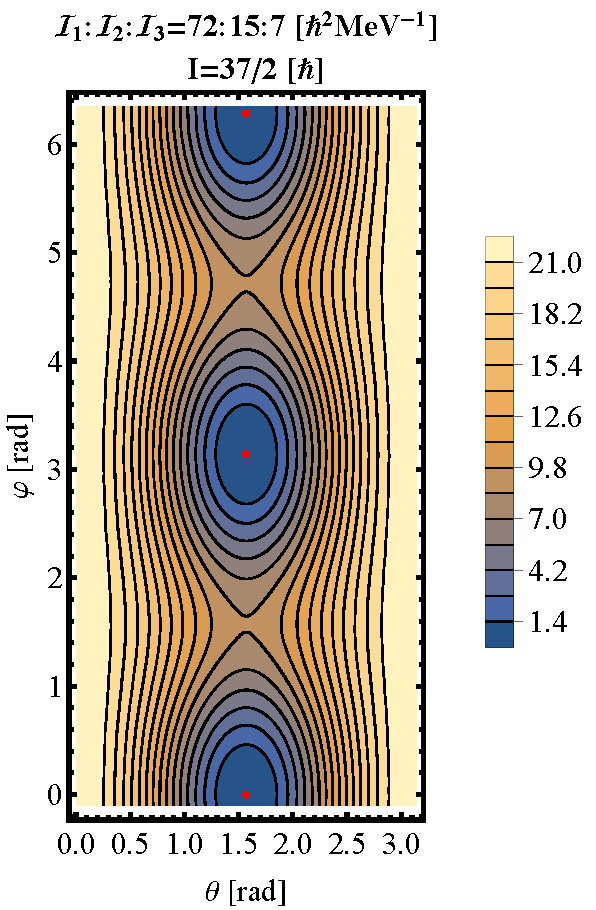
\includegraphics[scale=0.55]{images/contour-tsd3.pdf}
    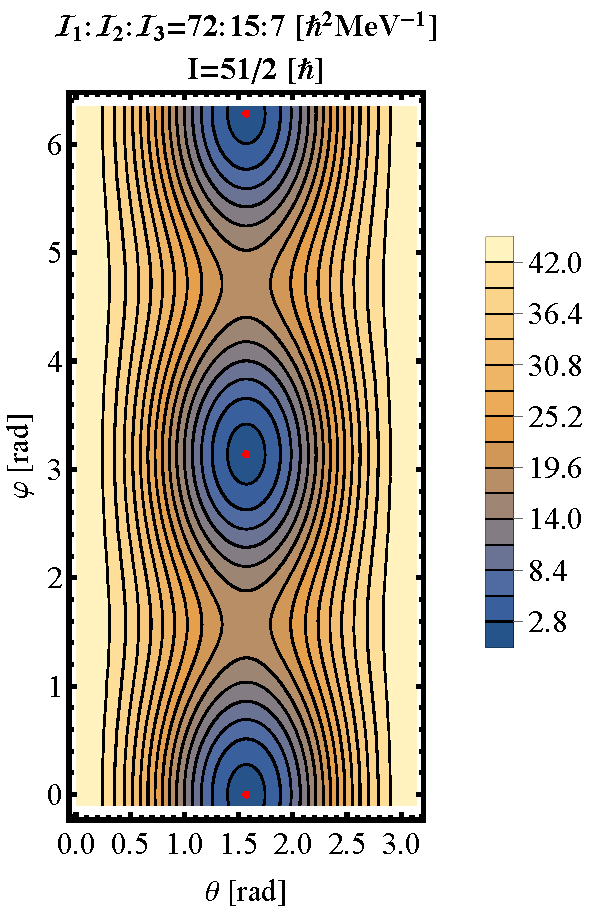
\includegraphics[scale=0.55]{images/contour-tsd4.pdf}
    \caption{A contour plot with the energy function $\mathcal{H}$ for TSD3 and TSD4. The parameter set $\mathcal{P}$ was used for the numerical calculations.}
    \label{contour-tsd3}
\end{figure}

% \begin{figure}
%     \centering
%     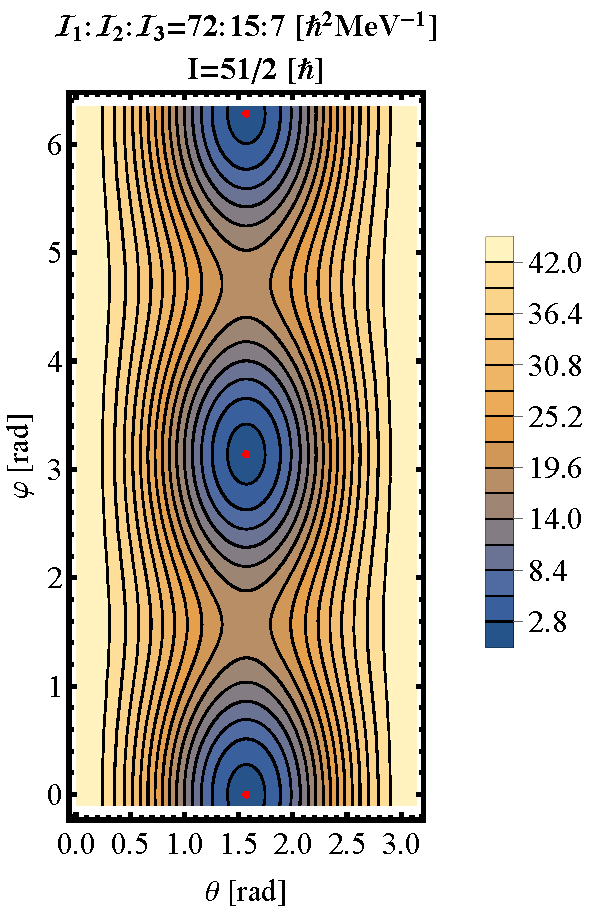
\includegraphics[scale=0.55]{images/contour-tsd4.pdf}
%     \caption{A contour plot with the energy function $\mathcal{H}$ for TSD4 with negative parity. The parameter set $\mathcal{P}$ was used for the numerical calculations.}
%     \label{contour-tsd4}
% \end{figure}

As a last step for the present model, an interest on finding the nuclear trajectories was given. The nuclear trajectories are graphically represented for a defined angular momentum for each band, within a 1x3 grid view. The three pictures that form a grid (where one grid corresponds to a triaxial band) represent trajectories of the system evaluated at certain spin $I$, but with different energy attributed to the triaxial ellipsoid E (see Eq. \ref{ellipsoid_rotation}). Namely, the first energy corresponds to the real excitation energy (obtained theoretically) for that particular spin state, the second one represents the point at which the ellipsoid touches the sphere at the equator - point which marks a nuclear phase transition - while the third one is the trajectory of the system at energies sufficiently large that the system changes its wobbling regime.

\begin{figure}
    \centering
    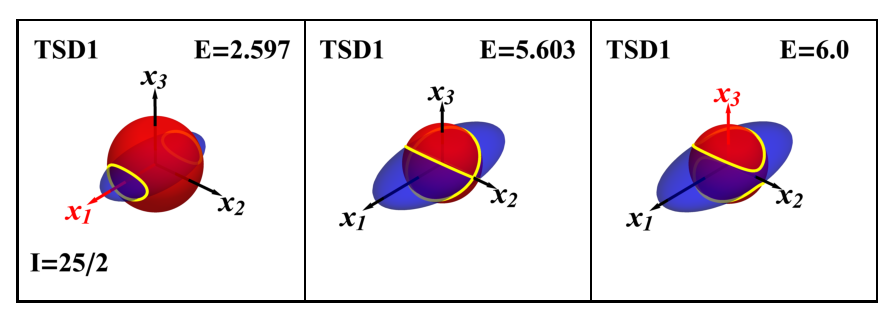
\includegraphics[scale=0.55]{images/tsd1_spin1.eps}
    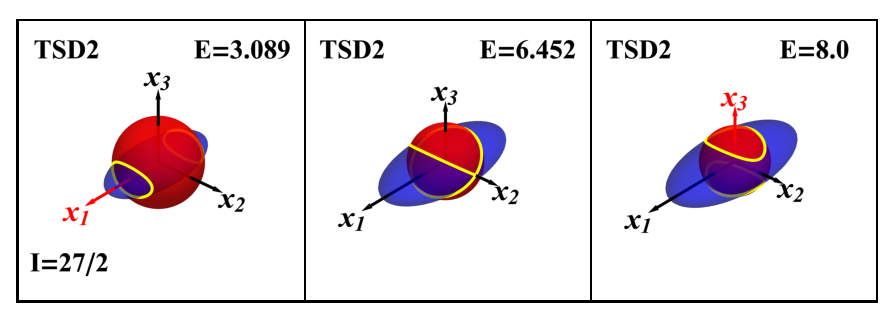
\includegraphics[scale=0.55]{images/tsd2_spin1.eps}
    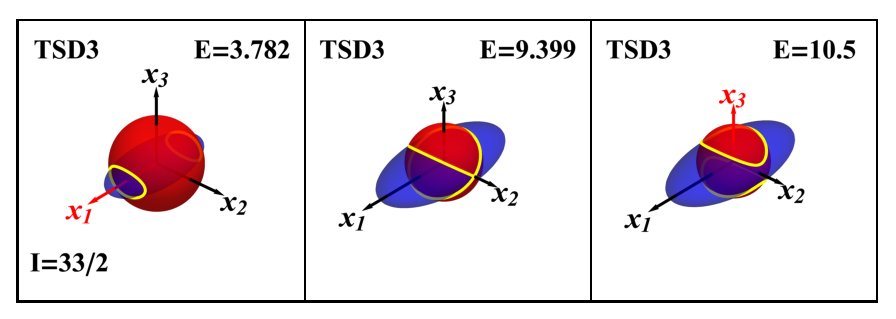
\includegraphics[scale=0.55]{images/tsd3_spin1.eps}
    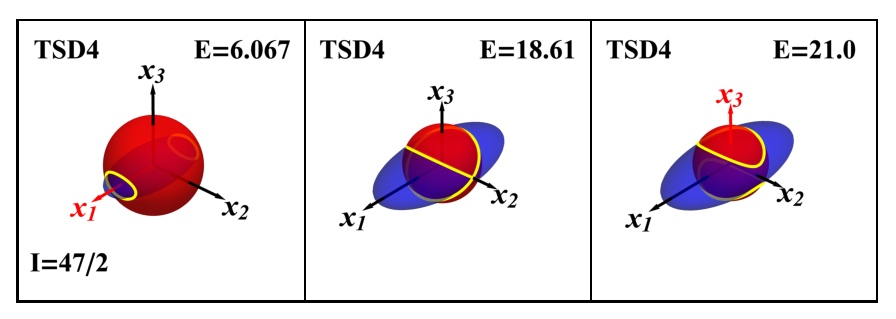
\includegraphics[scale=0.55]{images/tsd4_spin1.eps}
    \caption{The nuclear trajectory of the system for a spin state belonging to each of the four TSD bands of $^{163}$Lu. Intersection line marked with yellow color represents the actual orbits.}
    \label{ellipsoids-tsd1}
\end{figure}

Indeed, in Fig. \ref{ellipsoids-tsd1}, one can see the trajectory at which the nucleus rotates around the 1-axis (that is the axis with the largest moment of inertia), hinting towards a longitudinal wobbling character. On the other hand, there is a point at which the system undergoes a phase transition, where its axis of rotation changes from $x_1$ to that of $x_3$. The exact point where the phase transition takes place is represented by the yellow curves from the middle inset of the mentioned figures. Lastly, in the third inset element from the figures, a value of the total energy attributed to the energy ellipsoid is chosen sufficiently large, that the system changes its orientation - and therefore its wobbling regime - by making a shape transition. The transition from a longitudinal to a transverse wobbling is indeed forbidden, since the values of $E$ at which nucleus undergoes the change in rotation are larger than all the states that belong to any of the four bands: this can be seen in the third inset of each band from Fig. \ref{ellipsoids-tsd1}, where the energy at which system rotates around $x_3$ has an energy much larger than the one which corresponds at the given total angular momentum.

%\section{Conclusions}

Concluding, in the present study, a new interpretation for the structure of the wobbling bands within $^{163}$Lu isotope was developed, with the adoption of parity partner bands for TSD2 and TSD4. The meaning behind this is that now one can consider the same deformation parameters for TSD4 as for the rest of the family of triaxial bands. This is enforced by the similar spin sequences between TSD2 and TSD4, and because the coupling of the valence nucleon with the even-even core is considered to be uniform across both bands. Compared to the previously developed model \cite{raduta2020new}, the current results are improved in terms of agreement with the experimental data regarding the wobbling spectrum, but also it was possible to obtain the same MOI ordering (with $\mathcal{I}_1$ being the largest MOI). Results of the energy calculations was shown in Fig. \ref{wobbling_energies}, obtaining a fairly small deviation from the experimental data set.

The improved set of excitation energies resulted in a new parameter set $\mathcal{P}$ that is unique for the TSD bands. This allowed to continue investigating the energy function $\mathcal{H}_{min}$ of the system, obtained from the expansion of the initial expression of $\mathcal{H}$ around the minimum point. The function was graphically represented as contour plots, for each triaxial band, and its extremal values have been determined. Regions where the wobbling mode is stable can be found next to the minimum points. Within this interpretation of wobbling motion, a longitudinal-like character is obtained, however, as discussed in \cite{raduta2020new}, these are the effective MOIs obtained from the fitting procedure (with no spin-dependence upon them) so one cannot know for sure if this is the final picture, or indeed at some critical spin $I_c$ in the low-lying spectrum, there are nuclear phases where transverse character prevails. The contour plots for the four bands were shown in Figs. \ref{contour-tsd1} and \ref{contour-tsd3}.

Finally, the trajectories of the nuclear system were numerically determined through the intersection of the angular momentum sphere and the energy ellipsoid, evaluated for the parameter set $\mathcal{P}$ and a fixed angular momentum $I$. This is a major step in understanding the actual dynamics of a deformed even-odd nucleus such as $^{163}$Lu. A critical energy at which the system undergoes a phase transition, changing its rotation from precession around $x_1$ to $x_3$ was also pointed out.

Concluding, the present model is a successful tool for accurately describing the wobbling spectrum of ${163}$Lu, but also for understanding the rotational motion of the nuclear system with respect to its total spin.


%\section{Acknowledgments}

The first author wants to thank Prof. Raduta for the careful guidance throughout this work.

\bibliography{biblio}% Produces the bibliography via BibTeX.

\end{document}